\chapter{Lentilles gravitationnelles fortes de type galaxie-galaxie}\label{sec:lentilles gravitationnelles}

\thispagestyle{empty}


Fritz \citet{Zwicky1937}, suivant les calculs publiés par \citet{Einstein1936} et la première observation 
de l'effet de déviation gravitationnelle de la lumière par \citet{Eddington1919}, 
est largement reconnu comme étant le premier à observer correctement qu'une lentille gravitationnelle, et en particulier 
l'anneau d'Einstein \citep{Chwolson1924},
est un phénomène particulièrement riche en information\footnote{ 
        Les travaux pionniers de Franti\v{s}ek \citet{Link1936,Link1937}, largement ignorés dans la littérature anglo-saxonne, %\citep{Valls-Gabaud2006}, 
        offrent déjà une perspective riche et détaillée sur le phénomène des lentilles gravitationnelles au moment où \citet{Zwicky1937} publie 
        ses observations. 
        En particulier, \citet{Link1936} décrit la magnification d'une étoile lors du passage derrière un objet massif et 
        observe que les amas globulaires et les galaxies sont des candidats idéaux pour une recherche systématique du 
        phénomène.
        }. 
L'article de \citet{Zwicky1937} articule précisément deux idées centrales qui nous motivent encore aujourd'hui à 
étudier ces objets. En premier lieu, une lentille gravitationnelle est un télescope naturel, de sorte qu'un tel 
système nous permettrait en principe d'étudier l'image lentillée de la source en arrière-plan avec une résolution beaucoup plus grande que nos instruments 
nous le permettraient si l'effet de lentille n'avait pas eu lieu. En second lieu, la déflexion de l'image de la source 
est directement proportionnelle à la masse (gravitationnelle) de la lentille. 
\begin{equation}\label{eq:Taille Lentille}
        \theta_E = \sqrt{\frac{4 G M}{c^{2} D}} \simeq 3\left( \frac{M}{M_{\odot}} \right)^{\frac{1}{2}} \left( \frac{D}{1\, \mathrm{Gpc}} \right)^{-\frac{1}{2}}\, \mu\mathrm{as}\, , \hspace{1cm} \left\{D \equiv \frac{D_{\ell} D_s}{D_{\ell s}}\right\}\, .
\end{equation}
Par exemple, une galaxie typique de masse $M\sim 10^{11} M_{\odot}$, à une distance caractéristique $D= 3 \, \mathrm{Gpc}$ produirait des 
images de la source séparées par $2 \theta_E \sim 1''$. C'est cette observation qui intéressait particulièrement 
\citet{Zwicky1937b}, insatisfait par les méthodes pour mesurer la masse des nébuleuses extragalactiques (galaxies) 
de l'époque, basées largement sur des comparaisons de la luminosité totale de ces galaxies avec $L_\odot$, la luminosité du Soleil, 
ou des courbes de rotation képlériennes.\footnote{
\citet{Zwicky1937b} a estimé la masse de l'amas de Coma à $\gtrsim 4.5\times  10^{13}M_\odot$ avec le théorème du viriel. 
Cette limite inférieure est un très bon estimé de 
la valeur acceptée aujourd'hui, dérivée avec les effets de lentilles faibles produites par l'amas 
sur l'image des galaxies environnantes, soit $5^{+4.3}_{-2.1} \times 10^{14}\, h^{-1}_{70}\,M_\odot$\citep{Gavazzi2009}.
} 

\citet{Einstein1936} considérait l'éventualité d'observer ces systèmes comme étant extrêmement 
improbable, pointant vers les limitations instrumentales de l'époque. En effet, les télescopes terrestres étaient 
largement limités par l'effet de \textit{seeing} atmosphérique, soit la distorsion de l'image causée par la turbulence de 
l'atmosphère.

\begin{figure}[tb!]
        \centering
        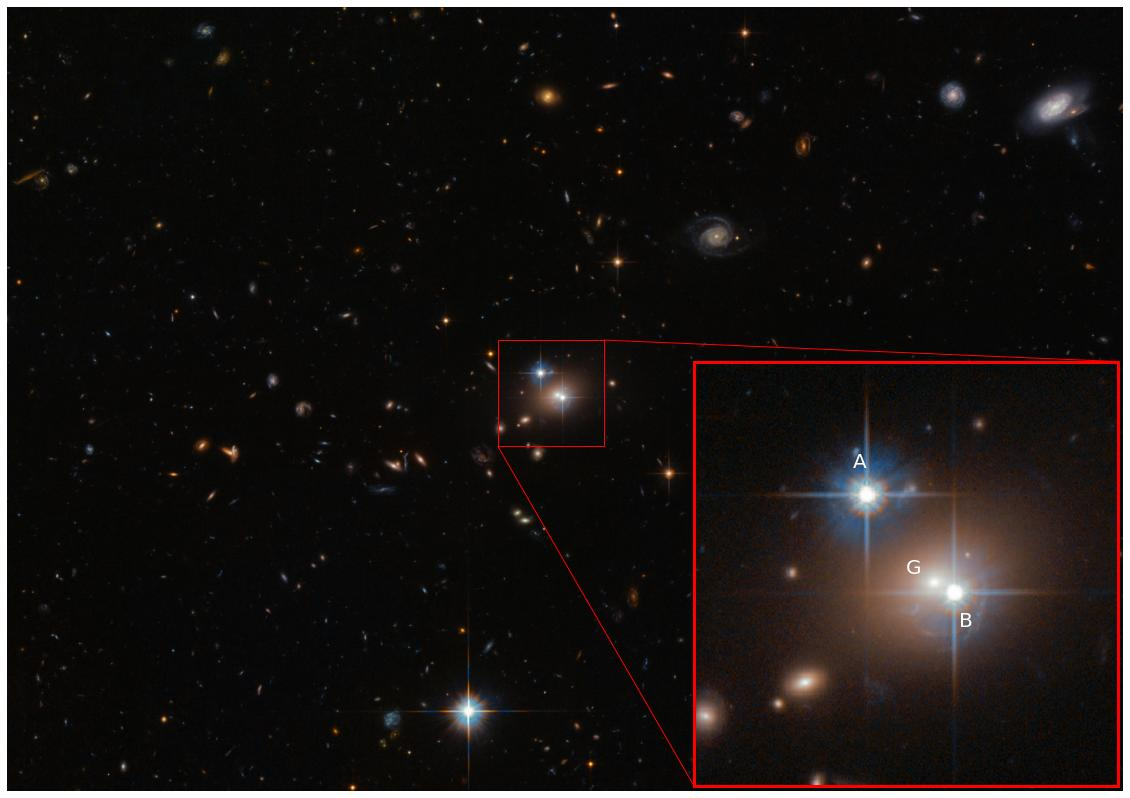
\includegraphics[width=0.8\textwidth]{figures/zoomed_in_qso0957}
        \caption{Le quasar double (QSO 0957+561 A et B) et la galaxie-lentille (G) imagée par le télescope spatial Hubble. 
        Crédit: ESA/Hubble et NASA, élargissement et annotation par AA.}
        \label{fig:doubel quasar}
\end{figure}

Dû à cette difficulté pratique, 
la première lentille gravitationnelle est découverte seulement plusieurs décennies après la prédiction de leur existence par \citet{Walsh1979}, 
suivant l'identification de deux spectres radios de quasars identiques, QSO 0957+561 A et B, séparés par $5.7$ secondes d'arcs
et capturés avec le télescope radio Mark II à l'observatoire Jodrell Bank. 
Les spectres partagent la même magnitude, $m=17$, le même décalage vers le rouge, $z=1.405$, et possèdent des détails 
chimiques suspicieusement semblables. Ces coïncidences suggèrent fortement que ces deux spectres sont des copies d'un seul objet, soit un noyau 
actif d'une galaxie en arrière-plan, produite par l'effet de lentille gravitationnelle d'une galaxie en avant-plan, invisible dans le 
domaine radio à une fréquence de $966\,\mathrm{MHz}$. Cette hypothèse est rapidement confirmée par 
l'observation optique de la galaxie-lentille ($z=0.355$) avec l'observatoire Palomar \citep{Young1980}\footnote{Simulténament 
observé et confirmé par le télescope de $2.2\, m$ de l'Université d'Hawaii au mont Mauna Kea \citep{Stockton1980}.}, 
ainsi que la modélisation de sa distribution de masse, de son environnement 
et des angles de déflexion qui causeraient l'apparition d'une image double du quasar \citep{Young1981,Falco1991}

À la suite de cette découverte fortuite, l'étude des lentilles gravitationnelles est devenue un sujet d'étude 
particulièrement riche et prometteur en cosmologie \citep{Blandford1992,Bartelmann2010,Treu2010}. 
Par exemple, les lentilles gravitationnelles permettent de mesurer 
la constante de \citet{Hubble1929}, $H_0$, qui quantifie le taux de l'expansion de l'Univers au temps présent. Les deux méthodes principales 
pour faire cette mesure à l'aide des lentilles gravitationnelles sont la caractérisation de la courbe de lumière des supernovas lentillées 
\citep{Refsdal1964,Kelly2015,Goobar2017} 
et la surveillance décennale de quasars lentillés 
\citep[e.g.][]{Vanderriest1989,Wong2020}. 



\begin{figure}[tb!]
        \centering
        \begin{subfigure}[t]{0.45\textwidth}
                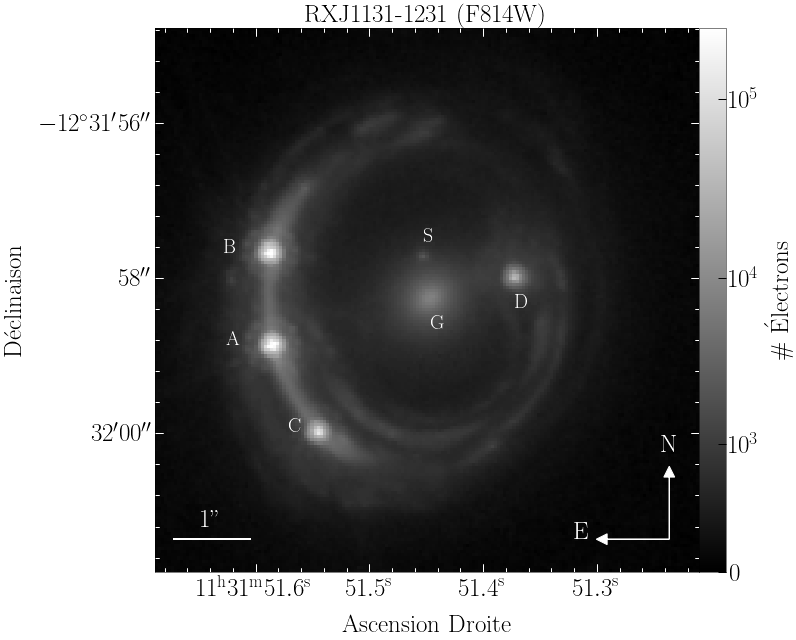
\includegraphics[width=\linewidth]{figures/rxj1131} 
                \caption{Quasar quadruplement lentillé (A, B, C et D) par une galaxie (G). L'image de la galaxie hébergeant le quasar 
                        est déformée tangentiellement, formant un anneau d'Einstein. Image prise par HST avec le filtre F814W.}
                \label{fig:rxj1131}
        \end{subfigure}
        ~
        \begin{subfigure}[t]{0.45\textwidth}
                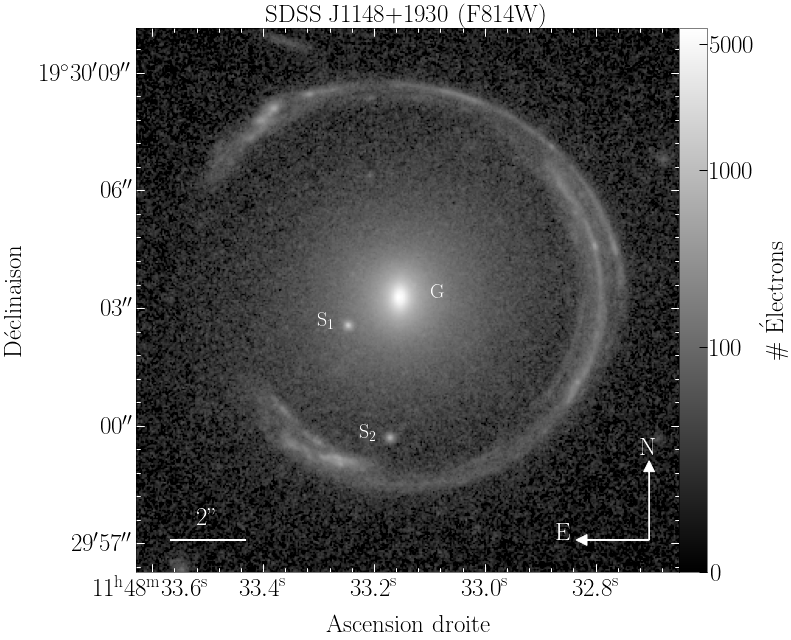
\includegraphics[width=\linewidth]{figures/sdssj1148} 
                \caption{Le fer à cheval cosmique, soit l'image d'une proto-galaxie à très haut décalage vers le rouge 
                        ($z=2.379$) fortement magnifiée et déformée par une galaxie elliptique lumineuse en infrarouge (G) exceptionnellement massive 
                        \citep[${5.2\times 10^{12}\, h_{72}^{-1}\, M_\odot}$,][]{Schuldt2019}. 
                 Image prise par HST avec le filtre F814W.}
                \label{fig:sdssj1148}
        \end{subfigure}
        \caption{Lentilles gravitationnelles de type galaxie-galaxie.}
        \label{fig:important lenses}
\end{figure}
 

De ce fait, plusieurs programmes ont été initiés pour trouver des lentilles gravitationnelles. Le programme 
\textit{Sloan Lens ACS Survey} \citep[SLAC,][]{Bolton2005,Bolton2006}, basé sur la recherche systématique de spectres de galaxies de type ETG\footnote{\textit{Early-Type Galaxies}} 
avec des lignes d'absorption à un décalage vers le rouge plus grand que les lignes d'émission, 
est un des programmes les plus réussis, ayant mené à la découverte 
confirmée de plus de $150$ lentilles gravitationnelles de type galaxie-galaxie \citep{Bolton2008,Shu2017}. Les programmes 
basés sur la recherche visuelle d'images doubles, triples, d'arcs ou d'anneaux \citep[e.g.][]{Faure2008} dans les 
champs du ciel larges et profonds comme 
COSMOS \citep{Koekemoer2007,Scoville2007}, connaissent aujourd'hui une renaissance nourrie par les succès récents de l'apprentissage profond 
pour la perception visuelle \citep{Krizhevsky2012}. Cette nouvelle approche a déjà mené à la découverte de plus de $1000$ lentilles 
gravitationnelles \citep{Petrillo2017,Huang2021}, et est projetée de découvrir plus de $10^{5}$ systèmes grâce 
aux nouveaux relevés du ciels prévus dans la prochaine décennie aux
observatoires Rubin \citep{lsst2009} et Euclid \citep{Euclid2010}.

%Le sujet du chapitre \ref{chap:censai} se concentre sur le défi de développer un algorithme pour modéliser la distribution de masse et 
%la morphologie de la source. Cet algorithme est dédié à analyser le nombre grandissant
%de lentilles gravitationnelles connues, dans toute leur complexité et dans un temps à l'échelle humaine. 
Dans la section qui suit, je dérive les équations centrales qui nous permettent 
d'étudier les lentilles gravitationnelles de type galaxie-galaxie.
Mon traitement est largement inspiré 
des manuels de références de \citet{Meneghetti2013,Congdon2018}. 


\section{Les angles de déflexion}

Supposons qu'un photon est sur une trajectoire parallèle à l'axe de 
visée $\mathbf{e}_{\parallel}$ d'un observateur sur Terre. 
Supposons de plus que la source d'un champ gravitationnel $\Phi$ est située sur l'axe de visée, 
ce qui a pour effet de courber la 
trajectoire de ce photon entre son point d'origine et son point d'arrivée.
On définit l'angle de déviation comme la déviation totale de cette trajectoire 
dans la direction perpendiculaire à l'axe de visée de l'observateur. 
De façon générale, cette déviation s'écrit
\begin{equation}\label{eq:intro alpha}
        \boldsymbol{ \alpha} = - \int_{\lambda_A}^{\lambda_B} \ddot{\mathbf{x}} \times \mathbf{e}_{\parallel} d\lambda\, ,
\end{equation}
où $\lambda$ paramétrise la trajectoire du photon $\mathbf{x}(\lambda)$. 
Le signe négatif nous indique qu'on prend la perspective de l'observateur. 

La trajectoire d'un photon obéit au 
principe de Fermat, qui stipule que la lumière suit une trajectoire qui extrémise
la durée du parcours entre deux points. 
Dans le langage du calcul 
des variations, la variation de la durée s'écrit
\begin{equation}\label{eq:Fermat}
        \delta T =  \delta \int_{A}^{B} n(\mathbf{x}(\ell)) \frac{d\ell}{c}= 0\, ,
\end{equation}
où $\ell$ est un élément de longueur sur la trajectoire et $n$ est un indice de réfraction.
Pour déterminer l'indice de réfraction du champ gravitationnel d'une galaxie, 
on doit utiliser le formalisme de la relativité générale. Selon le principe 
d'équivalence (fort), 
l'effet d'un champ gravitationnel est localement 
indistinguable d'une accélération causée par la courbure 
d'un espace-temps décrit par 
une métrique $g_{\mu \nu}$. 
La trajectoire d'un photon se trouve alors en cherchant 
les géodésiques de cet espace-temps. 
On fait l'approximation 
que le potentiel $\Phi$ d'une galaxie est celui d'un gaz parfait, c'est-à-dire 
qu'il satisfait une équation de Poisson
\begin{equation}\label{eq:Poisson}
       \grad^{2}\Phi = 4\pi G \rho .
\end{equation} 
Dans la limite où ce potentiel est faible $\displaystyle \frac{2\Phi}{c^{2}} \ll 1$, la 
métrique $g_{\mu \nu}$ est décrite par une expansion au premier ordre autour de la 
métrique de Minkowsky %$\eta_{\mu\nu}$
\begin{equation}\label{eq:metrique}
        ds^2 = g_{\mu\nu}dx^{\mu}dx^{\nu} \approx \left( 1 + \frac{2\Phi}{c^{2}} \right)c^{2}dt^{2} - \left( 1 - \frac{2\Phi}{c^{2}} \right)d\mathbf{x}^{2}.
\end{equation} 
Puisqu'un photon suit une géodésique de l'espace-temps $ds^{2} = 0$, on peut déterminer 
l'indice de réfraction en réarrangeant l'équation \eqref{eq:metrique}
\begin{equation}\label{eq:n}
        n \equiv c \left( \frac{\lVert d \mathbf{x} \rVert}{dt}  \right)^{-1} \approx  1 - \frac{2\Phi}{c^{2}}.
\end{equation} 
En réécrivant l'élément de longueur $d\ell$ en termes du 
paramètre de la trajectoire
$
        d\ell = \left\lVert\frac{d  \mathbf{x} }{d\lambda} \right\rVert d\lambda,
$
on peut réécrire l'équation \eqref{eq:Fermat} sous la forme
\begin{equation}\label{eq:Fermat2}
        \delta \int_{\lambda_A}^{\lambda_B} n(\mathbf{x}) \lVert \mathbf{\dot{x}} \rVert d\lambda = 0.
\end{equation} 
Par correspondance avec la fonctionnelle de l'action 
$J(x) = \int_{\lambda_0}^{\lambda_1} \mathcal{L}(\lambda,\, x,\,\dot{x}) d\lambda$, on trouve que 
le lagrangien de la trajectoire s'écrit 
$
        \mathcal{L} = n(\mathbf{x})  \sqrt{\dot{x}^{2}}.
$
La trajectoire qui satisfait \eqref{eq:Fermat} 
est une solution des équations d'Euler-Lagrange
\begin{equation}\label{eq:EulerLagrange}
        \frac{d }{d \lambda} \frac{\partial \mathcal{L}}{\partial \dot{\mathbf{x}}} - \frac{\partial \mathcal{L}}{\partial \mathbf{x}} = 0.
\end{equation} 
On a donc
\begin{equation}\label{eq:EulerLagrange2}
        \frac{d }{d \lambda} n \frac{\dot{\mathbf{x}}}{\lVert \dot{\mathbf{x}} \rVert}- \lVert \dot{\mathbf{x}} \rVert \grad n = 0 ,
\end{equation} 
Puisque le choix du paramètre $\lambda$ est libre, on peut le choisir tel 
que $\lVert \dot{\mathbf{x}} \rVert = 1$ en tout point de la trajectoire. Ainsi,
\begin{align}
        \nonumber
        \frac{d }{d \lambda} n \dot{\mathbf{x}} -  \grad n &= 0 \\
\label{eq:EulerLagrange3}
        \implies n \ddot{\mathbf{x}} + (\grad n \cdot \dot{\mathbf{x}}) \dot{\mathbf{x}} - \grad n &= 0
\end{align} 

À ce point de la dérivation, on utilise l'approximation de Born. 
C'est-à-dire qu'on approxime la trajectoire 
du photon comme une ligne droite sur l'axe de visée $\mathbf{e}_{\parallel}$. 
Cette approximation est justifiée 
dans le contexte des lentilles gravitationnelles de type galaxie-galaxie, 
puisque les angles de déviation sont généralement de 
l'ordre de l'arcseconde ou plus petits. 
Comme le vecteur $\dot{\mathbf{x}}$ est tangent à la trajectoire du photon, les termes $ \propto \dot{\mathbf{x}} \times \mathbf{e}_{\parallel} $ s'annulent. 
En subsitutuant l'indice de réfraction par \eqref{eq:n} dans $\mathbf{e}_{\parallel} \times \eqref{eq:EulerLagrange3}$, on obtient
\begin{equation}\label{eq:sol}
        \ddot{\mathbf{x}} \times \mathbf{e}_{\parallel} = \frac{1}{n} \grad_\perp n = \grad_\perp \log n
        \approx -\frac{2}{c^{2}}\grad_{\perp} \Phi\,,
\end{equation} 
où $\grad_\perp$ est un gradient selon les coordonnées perpendiculaires à $\mathbf{e}_\parallel$.
On note que le facteur 2 qui apparaît dans l'équation \eqref{eq:sol} est un 
effet qui vient de la relativité générale. Ce facteur corrige la solution 
que l'on aurait obtenue avec une dérivation classique (newtonienne).


On est maintenant en mesure de calculer l'angle de déviation. 
J'introduis le paramètre d'impact $\boldsymbol{\xi}$ qui est la distance perpendiculaire entre 
la position d'origine du photon sur le plan de la lentille  
et l'axe de visée (voir Figure \ref{fig:cartoon}).
Dans le cas où le potentiel est généré par une masse $M$ ponctuelle, c.-à-d.\ qu'on 
suppose $\rho = M\delta^{3}(\mathbf{x})$, où $\delta $ est la fonction delta de Dirac, 
alors le potentiel qui satisfait l'équation de Poisson \eqref{eq:Poisson} est 
la fonction de Green 
$\displaystyle \Phi = -\frac{GM}{\sqrt{ \xi^{2} + z^{2}}}$, où $z$ est la coordonnée 
sur l'axe de visée. L'équation \eqref{eq:intro alpha} se réécrit finalement comme 
\begin{align}
\nonumber
        \boldsymbol{ \alpha}(\boldsymbol{ \xi} ) &= -\frac{2GM}{c^{2}} \int_{-\infty }^{\infty }  \frac{\partial}{\partial \boldsymbol{\xi} }\frac{1}{(\xi^{2} + z^{2})^{1/2}}dz \\
\label{eq:deflection approx}
        \implies \boldsymbol{ \alpha}(\boldsymbol{ \xi})  &= \frac{4GM}{c^{2}  \xi^{2} } \boldsymbol{ \xi}
\end{align} 
Cette solution se généralise naturellement à un profil de masse quelconque en assumant 
qu'il s'exprime comme une somme d'éléments de masse $dm = \Sigma d^{2}\boldsymbol{ \xi}'$, 
où $\Sigma = \int \rho dz$ est une densité surfacique de masse. 
L'angle de déviation total mesuré à un point $\boldsymbol{\xi} $ est alors une convolution 
sur tout le plan de la lentille (mince) puisque l'équation \eqref{eq:deflection approx} dépend 
linéairement de la masse $M$:
\begin{equation}\label{eq:alpha physique}
        \boldsymbol{ \alpha} (\boldsymbol{ \xi} ) = \frac{4 G}{c^{2}} 
        \int_{\mathbb{R}^{2}} \Sigma (\boldsymbol{ \xi} ')
        \frac{\boldsymbol{ \xi}  - \boldsymbol{ \xi} '}{\lVert \boldsymbol{ \xi}  - \boldsymbol{ \xi} ' \rVert^{2}}d^{2}\boldsymbol{ \xi} '
\end{equation} 

\begin{figure}[tb!]
        \centering
        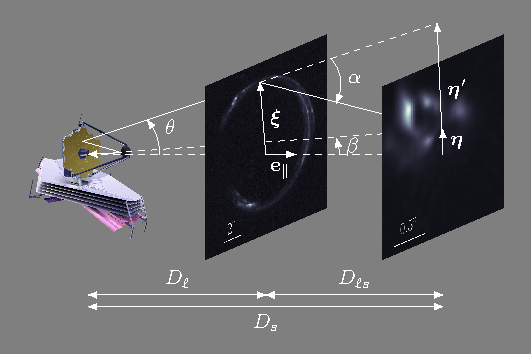
\includegraphics[width=0.8\textwidth]{figures/lensing_cartoon}
        \caption{Schéma d'une lentille gravitationnelle.}
        \label{fig:cartoon}
\end{figure}

L'angle de déviation est une quantité cruciale pour résoudre une lentille gravitationnelle 
puisqu'il décrit une transformation des coordonnées angulaires du plan de la lentille ($\boldsymbol{ \theta} $) 
vers les coordonnées angulaires du plan de la source ($\boldsymbol{ \beta} $). 
On assume que les distances entre l'observateur et la lentille $D_{\ell}$, entre l'observateur et la source $D_s$ et entre la lentille et la source $D_{\ell s}$, 
sont beaucoup plus grandes que les distances perpendiculaires à l'axe de visée $\boldsymbol{ \xi} $ ou $\boldsymbol{ \eta}$ 
(voir figure \ref{fig:cartoon}). 
Cette approximation est justifiée pour les objets qui nous intéressent,
pour lesquels les distances parallèles à l'axe de visée sont généralement 
de l'ordre du Gpc, alors que les distances perpendiculaires sont généralement 
de l'ordre du kpc; soit 6 ordres de grandeur de différence.
Ainsi, on peut faire un argument géométrique (euclidien) 
\begin{align}
\nonumber
       D_{s} \boldsymbol{ \theta} &= \boldsymbol{ \eta}' \\   
\nonumber
       D_{s} \boldsymbol{ \beta} &= \boldsymbol{ \eta} \\   
\nonumber
       D_{\ell s} \boldsymbol{ \alpha} &= \boldsymbol{ \eta}' - \boldsymbol{ \eta}  \\   
\label{eq:lens equation}
       \implies D_s \boldsymbol{ \beta} &= D_s \boldsymbol{ \theta} - D_{\ell s} \boldsymbol{ \alpha}   
\end{align} 
La dernière relation est l'équation maîtresse qui nous permet de tracer les rayons lumineux d'une source 
vers un détecteur fictif dans nos simulations. 

On notera que cette relation reste valide pour un Univers courbe et/ou en expansion 
(c.-à-d.\ décrit par une géométrie non euclidienne), 
à condition qu'on utilise une notion de distance qui satisfait, par définition, la relation trigonométrique euclidienne
\begin{equation}\label{eq:diameter angular distance}
       D \equiv \frac{\xi}{\theta}\, ,
\end{equation} 
où $\xi$ est la taille physique d'un objet placé à une certaine distance de l'observateur, et $\theta$ est l'angle solide sous-tendu 
par cet objet. Pour un Univers décrit par la métrique de Friedmann-Lemaître-Robertson-Walker,
la notion de distance qui respecte la définition \eqref{eq:diameter angular distance} est la distance du diamètre angulaire. 
En pratique, on peut exprimer $D$ en termes du décalage vers le rouge des photons émis par l'objet, $z$. 
On note $a(z)$ le facteur d'échelle lorsque le photon est émis par la source et $a(0)$ le facteur d'échelle au moment présent ($z=0$).
Pour un Univers plat \citep[voir les manuels de référence][]{Coles2002,Dodelson2003,Bartelmann2004}
\begin{align}
        D_z &= c a(z) \underbrace{\int_{a(z)}^{a(0)} \frac{da}{a \dot{a}}}_{\strut\mathclap{\text{distance comobile}}}; \\[2ex]
                \nonumber
              &= \frac{c a(z)}{H_0} \int_{a(z)}^{a(0)} \frac{da}{\sqrt{\Omega_{r,0} + \Omega_{m,0} a  + \Omega_{\Lambda,0}a^{4}}}; \\
              \label{eq:dang}
              &= \frac{c}{H_0(1 + z)} \int_{0}^{z} \frac{dz'}{\sqrt{\Omega_{r,0}(1 + z')^{4} + \Omega_{m,0} (1 + z')^{3} + \Omega_{\Lambda,0} }}\, .
\end{align}
On a utilisé la relation entre le facteur d'échelle, $a$, et le décalage vers le rouge, $a = (1 + z)^{-1}$, pour obtenir l'équation \eqref{eq:dang} 
par un changement de la variable d'intégration. 
$\Omega_{r,0}$, $\Omega_{m,0}$ et $\Omega_{\Lambda, 0}$ sont les paramètres de densités, au temps présent, de la radiation, de la matière et de l'énergie sombre 
respectivement. 
%$\Omega_K = 1 - \Omega_0$ est le paramètre de courbure et 
$H_0$ est la constante de Hubble, soit le taux 
d'expansion de l'Univers au temps présent. La distance $D_{\ell s}$ se trouve simplement en ajustant les bornes de l'intégrale $\int_0^{z} \mapsto \int_{z_\ell}^{z_s}$.
La valeur des paramètres du modèle cosmologique $\Lambda$CDM obtenue par l'équipe \citet{PlanckCollaboration2018}
est rapportée dans l'annexe \ref{app:lcdm}.


Il est généralement pratique de travailler avec la forme adimensionnelle de l'équation \eqref{eq:lens equation}. 
On introduit la densité critique 
\begin{equation}\label{eq:densite critique}
        \Sigma_c = \frac{c^2}{4 \pi G}\frac{D_{s}}{D_{\ell s} D_\ell}\, ,
\end{equation} 
qui nous permet de définir la quantité qu'on nomme convergence $\displaystyle \kappa(\boldsymbol{ \theta} ) \equiv \frac{\Sigma(\boldsymbol{ \theta})}{\Sigma_c}$. 
On définit ainsi l'angle réduit 
\begin{equation}\label{eq:alpha adim}
        \hat{\boldsymbol{ \alpha}} (\boldsymbol{ \theta}) = \frac{1}{\pi}\int_{\mathbb{R}^{2}} \kappa(\boldsymbol{ \theta} )
        \frac{\boldsymbol{ \theta} - \boldsymbol{ \theta}'  }{\lVert \boldsymbol{ \theta} - \boldsymbol{ \theta}' \rVert  } d^{2}\boldsymbol{ \theta}'\, ,
\end{equation} 
qui satisfait l'équation de la lentille adimensionnelle 
\begin{equation}\label{eq:lens equation adim}
        \boldsymbol{ \beta} = \boldsymbol{ \theta} - \hat{\boldsymbol{ \alpha}}(\boldsymbol{ \theta})\, . 
\end{equation}

Les équations \eqref{eq:alpha adim} et \eqref{eq:lens equation adim} sont les équations centrales à 
la modélisation des lentilles gravitationnelles. Elles sont utilisées pour simuler des lentilles 
gravitationnelles au chapitre \ref{chap:censai}. Elles sont aussi utilisées pour résoudre le 
problème inverse qui consiste à inférer l'image non-distordu de la galaxie en arrière-plan, $I(\boldsymbol{ \beta})$, 
et les paramètres de la distribution de masse de la galaxie-lentille, $\kappa(\boldsymbol{ \theta})$,
à partir des distortions observées de l'image en arrière-plan $I(\boldsymbol{ \theta})$. 
%soit le problème inverse qui motive la recherche présentée dans ce mémoire.

